% CV Customer Service Forwarding -- bien dich bang XeLaTeX.
% Dat anh portrait_CV.jpg cung thu muc voi file .tex.
\documentclass[10pt,a4paper]{article}
\usepackage{fontspec}
\defaultfontfeatures{Ligatures=TeX}
\IfFontExistsTF{Noto Sans}{\setmainfont{Noto Sans}}{\setmainfont{DejaVu Sans}}
\usepackage[a4paper,left=1.65cm,right=1.65cm,top=1.40cm,bottom=1.45cm]{geometry}
\usepackage[unicode,hidelinks]{hyperref}
\usepackage{graphicx}
\usepackage{tikz}
\usepackage{xcolor}
\usepackage{enumitem}
\usepackage{needspace}
\usepackage{ragged2e}
\definecolor{ink}{HTML}{1E2C36}
\definecolor{slate}{HTML}{344F61}
\definecolor{muted}{HTML}{59646D}
\definecolor{rule}{HTML}{CED6DB}
\pagestyle{empty}
\setlength{\parindent}{0pt}
\setlength{\parskip}{0pt}
\setlength{\emergencystretch}{2em}
\urlstyle{same}
\AtBeginDocument{\fontsize{10.25}{16}\selectfont\RaggedRight\color{ink}}
\setlist[itemize]{leftmargin=1.28em,topsep=5pt,itemsep=6pt,parsep=0pt,partopsep=0pt}

\newif\ifcvphoto
\cvphototrue

\newcommand{\cvsection}[1]{%
  \par\vspace{15pt}\needspace{4\baselineskip}%
  {\color{slate}\bfseries\fontsize{11.9}{14}\selectfont #1}\par\vspace{5pt}%
  {\color{rule}\hrule height 0.65pt}\vspace{7pt}%
}
\newcommand{\cvjob}[3]{%
  {\bfseries #1}\hfill {\color{muted}\fontsize{9.4}{12.3}\selectfont #2}\par\vspace{2pt}%
  {\color{muted}#3}\par%
}
\newcommand{\cvheading}{%
  {\color{ink}\bfseries\fontsize{19}{24}\selectfont NGUYỄN THỊ MINH TÂM}\par\vspace{4pt}%
  {\bfseries\color{slate}\fontsize{12.8}{15}\selectfont CUSTOMER SERVICE}\par\vspace{12pt}%
  {\fontsize{10.2}{14.5}\selectfont
  TP. Hồ Chí Minh \enspace\textbullet\enspace 0858662582\par\vspace{2pt}%
  \href{mailto:ngthiminhtam1904@gmail.com}{ngthiminhtam1904@gmail.com}}%
}

% Can chinh anh tron: sua photoZoom/photoX/photoY (don vi cm).
% Dung anh portrait_CV.png theo ti le goc, khong ep chieu ngang/doc.
\newcommand{\cvportrait}{%
  \begin{tikzpicture}
    \def\radius{1.5}
    \def\photoZoom{2.79cm}
    \def\photoX{0.08cm}
    \def\photoY{-0.17cm}
    \path[use as bounding box] (-\radius,-\radius) rectangle (\radius,\radius);
    \clip (0,0) circle (\radius cm);
    \node[inner sep=0] at (\photoX,\photoY) {%
      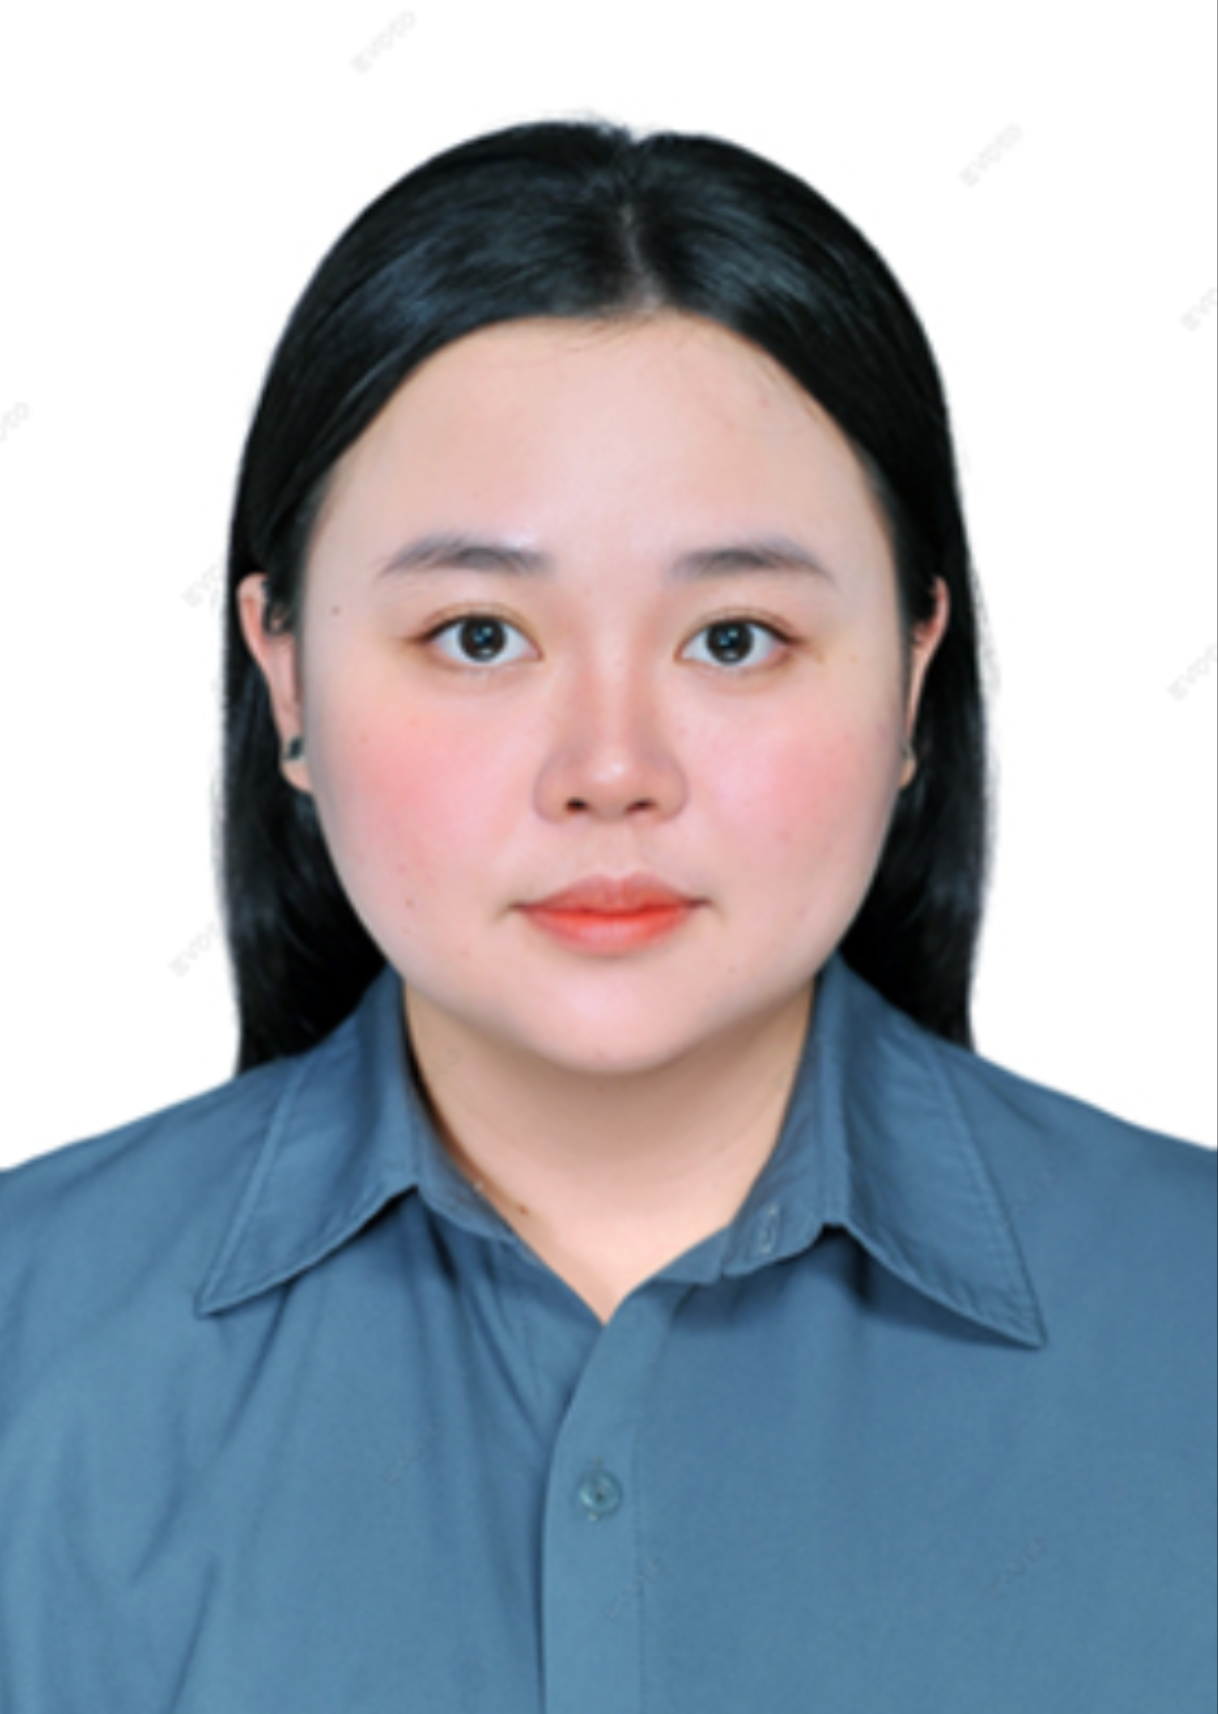
\includegraphics[width=\photoZoom]{portrait_CV.png}%
    };
  \end{tikzpicture}%
}

\begin{document}
\ifcvphoto
  \IfFileExists{portrait_CV.png}{%
    \noindent\begin{minipage}[t]{0.76\linewidth}
      \vspace{0pt}\cvheading
    \end{minipage}\hfill%
    \begin{minipage}[t]{0.19\linewidth}
      \vspace{0pt}\raggedleft\cvportrait
    \end{minipage}\par
  }{\cvheading\par}
\else
  \cvheading\par
\fi

\cvsection{GIỚI THIỆU}
Cử nhân Kinh doanh quốc tế, chuyên ngành Logistics \& Supply Chain Management, có kinh nghiệm thực tập Customer Service tại doanh nghiệp giao nhận vận tải. Đã tham gia theo dõi booking, lịch tàu và phối hợp với hãng tàu, đại lý. Từng làm Sales Express, có kinh nghiệm tư vấn và hỗ trợ khách hàng trong ngành logistics.

\cvsection{KINH NGHIỆM LÀM VIỆC}
\cvjob{Thực tập sinh Customer Service}{08/2026 -- Hiện tại}{Super Cargo Service (SCS)}
\begin{itemize}
    \item Theo dõi, hỗ trợ xử lý booking, bao gồm điều chỉnh thông tin, đổi lịch tàu, hủy và khôi phục booking.
    \item Cập nhật ETD, tàu/chuyến và thông tin lô hàng; kiểm tra thời hạn SI/VGM khi có thay đổi lịch trình.
    \item Phối hợp với hãng tàu và đại lý để đối chiếu, xác nhận booking và giải quyết vấn đề phát sinh.
  % Xac nhan tung tac vu duoi day voi ung vien truoc khi nop CV.
  \item Đọc hiểu email nghiệp vụ tiếng Anh liên quan đến booking và lịch trình vận chuyển.
  \item Tra cứu lịch tàu, trạng thái booking qua cổng thông tin hãng tàu.
  \item Cập nhật dữ liệu và trạng thái lô hàng trên hệ thống quản lý nội bộ.
\end{itemize}

\vspace{8pt}
\cvjob{Sales Express}{09/2025 -- 11/2025}{THD Logistics Việt Nam}
\begin{itemize}
   \item Tìm kiếm và tư vấn khách hàng có nhu cầu sử dụng dịch vụ logistics; giải đáp thông tin về dịch vụ.
  \item Chăm sóc khách hàng, phối hợp theo dõi đơn hàng và xử lý các yêu cầu phát sinh.
\end{itemize}

\vspace{8pt}
\cvjob{Nhân viên bán hàng}{03/2023 -- 06/2023}{WinMart -- WinCommerce}
\begin{itemize}
  \item Tư vấn khách hàng và hỗ trợ kiểm tra hàng hóa, tình trạng tồn kho tại cửa hàng.
\end{itemize}

\cvsection{HỌC VẤN}
\textbf{Đại học Tài chính -- Marketing}\hfill {\color{muted}\fontsize{9.4}{12.3}\selectfont 2022 -- 2025}\par\vspace{3pt}
Cử nhân Kinh doanh quốc tế, chuyên ngành Logistics \& Supply Chain Management\par\vspace{2pt}
GPA: 3.2/4.0

\cvsection{CHỨNG CHỈ VÀ NGOẠI NGỮ}
\textbf{MOS Excel:} 978/1000 \enspace\textbullet\enspace \textbf{MOS Word:} 962/1000 \enspace\textbullet\enspace \textbf{IELTS Academic:} 5.5


\end{document}
